%This is a template for producing OASIcs articles.
%See oasics-manual.pdf for further information.

\documentclass[a4paper,UKenglish]{oasics}
  %for A4 paper format use option "a4paper", for US-letter use option "letterpaper" for british
  %hyphenation rules use option "UKenglish", for american hyphenation rules use option "USenglish"

\usepackage{microtype}%if unwanted, comment out or use option "draft"
\usepackage{hyperref}
\lstset{
  basicstyle=\footnotesize,        % the size of the fonts that are used for the code
}

%\graphicspath{{./graphics/}}%helpful if your graphic files are in another directory

\bibliographystyle{plain}% the recommended bibstyle

% Author macros %%%%%%%%%%%%%%%%%%%%%%%%%%%%%%%%%%%%%%%%%%%%%%%%
\newcommand{\abc}{\textsc{abc}}
\newcommand{\abcpt}{\abc{} processing tool}
\newcommand{\abcdt}{\textsc{abc::dt}}
\newcommand{\midi}{\textsc{midi} }
\newcommand{\toabc}{\emph{toabc}}
\newcommand{\abcprocessor}{\emph{abc\_processor}}
\newcommand{\abcmtops}{\texttt{abcm2ps}}
\newcommand{\abctomidi}{\texttt{abc2midi}}
\newcommand{\awk}{\texttt{awk} }

\title{ABC with a UNIX flavor}
\titlerunning{ABC with a UNIX flavor} 
  %optional, in case that the title is too long; the running title should fit into the top page
  %column

\author[1]{Bruno M. Azevedo}
\author[2]{J. João Almeida}
\affil[1]{Department of Informatics, Universidade do Minho\\
  Portugal\\
\texttt{pg19819@alunos.uminho.pt}}
\affil[2]{Department of Informatics, Universidade do Minho\\
  Portugal\\
\texttt{jj@di.uminho.pt}}
\authorrunning{B. M. Azevedo}
  %mandatory. First: Use abbreviated first/middle names. Second (only in severe cases): Use first
  %author plus 'et. al.'

\Copyright{Bruno M. Azevedo}
  %mandatory. OASIcs license is "CC-BY";  http://creativecommons.org/licenses/by/3.0/

\subjclass{H.5.5 Sound and Music Computing, D.3.4 Processors - Compilers}
  % mandatory: Please choose ACM 1998 classifications from http://www.acm.org/about/class/ccs98-html
  %. E.g., cite as "F.1.1 Models of Computation". 
\keywords{Music Processing, ABC Notation, Unix, Scripting, Compilers}% mandatory: Please provide 1-5 keywords
%%%%%%%%%%%%%%%%%%%%%%%%%%%%%%%%%%%%%%%%%%%%%%%%%%%%%%%%%

%Editor-only macros (do not touch as author)%%%%%%%%%%%%%%%%%%%%%%%%%%%%%%%%%%%
\serieslogo{}%please provide filename (without suffix)
\volumeinfo%(easychair interface)
{Billy Editor, Bill Editors}% editors
{2}% number of editors: 1, 2, ....
{Conference/workshop/symposium title on which this volume is based on}% event
{1}% volume
{1}% issue
{1}% starting page number
\EventShortName{}
\DOI{10.4230/OASIcs.xxx.yyy.p}% to be completed by the volume editor
%%%%%%%%%%%%%%%%%%%%%%%%%%%%%%%%%%%%%%%%%%%%%%%%%%%%%%%%%

\begin{document}

\maketitle
\begin{abstract}
\abc{}~\cite{abcnotation:Online} is a simple, yet powerful, textual musical notation.\\
This paper presents \abcdt{}, a rule-based domain-specific
language~\cite{kosar2010comparing,kosar2008preliminary} (Perl embedded), designed to simplify the
creation of \abcpt{}s. Inspired by the Unix philosophy, those tools intend to be
simple and compositional in a Unix filters' way.\\
From \abcdt{}'s rules we obtain an \abcpt{} whose main algorithm follows a traditional
compiler architecture, thus consisting of three stages: 1) \abc{} parser (based on
\abcmtops'~\cite{abcm2ps:Online} parser), 2) \abc{} semantic transformation (associated with \abc{}
attributes), 3) output generation (either a user defined or system provided \abc{} generator).
\end{abstract}

\section{Introduction}
As computers were introduced to the world of music, a variety of file formats and textual notations
emerged in order to describe music, such as, \abc, LilyPond~\cite{lilypond:Online} or
MusicXML~\cite{musicxml:Online}.

\abc{} is used as the base notation throughout all of this paper. Listing \ref{lst:verbum_s1_p1}
illustrates an example of \abc{} notation and figure \ref{fig:verbum_s1_p1_score} its corresponding
score.\\

\lstinputlisting[caption={Verbum caro factum est: Section 1; Part 1 - Soprano},label={lst:verbum_s1_p1},captionpos=t,abovecaptionskip=-\medskipamount]{misc/verbum_s1_p1.tex}

\vspace{-0.25cm}
\begin{figure}[htb]
  \centering 
  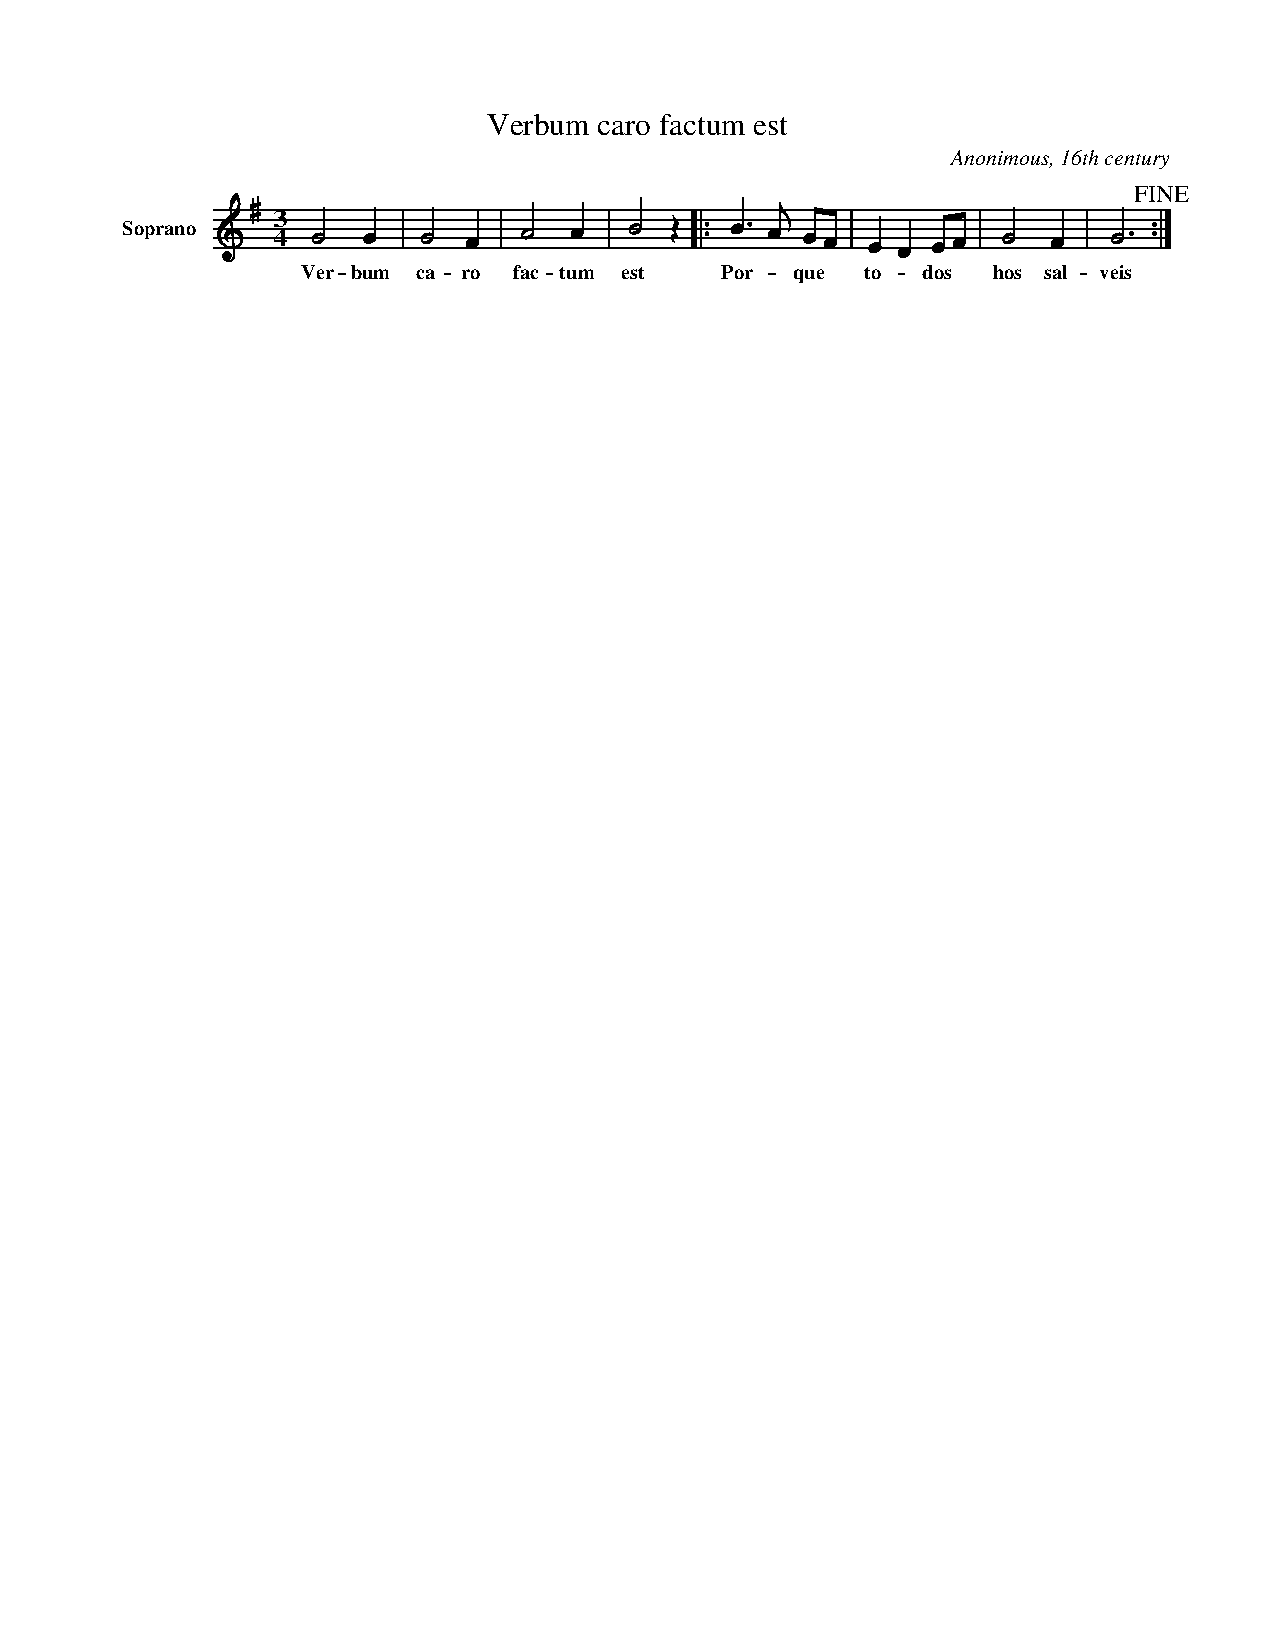
\includegraphics[width=0.8\textwidth, clip=true, trim = 0mm 230mm 0mm 17mm]{img/101.pdf} 
  \caption{Verbum caro factum est Score: Sections 1: Part 1 - Soprano}
  \label{fig:verbum_s1_p1_score}
\end{figure}

There are many \abcpt{}s and, among them, the most popular are the
\abcmtops{}~\cite{abcm2ps:Online} typesetter and the \midi creator
\abctomidi~\cite{abc2midi:Online}. The first translates music written in \abc{} into customary sheet
music scores in PostScript or SVG format. The latter converts an \abc{} file into a \midi file.

\subsubsection*{UNIX Metaphor}

The Unix philosophy~\cite{raymond2004art} emphasizes the creation of simple, yet capable and
efficient programs, which tackle only one problem at a time. Moreover, programs should handle text
streams as a universal type. The latter allows programs to easily communicate with each other.

In order to facilitate the development of new Unix commands, Unix creators built a new language (C).

\begin{quotation}
  \small\textit{Unix is simple. It just takes a genius to understand its simplicity.}
  \begin{flushright}
    Dennis Ritchie
  \end{flushright}
\end{quotation}

When we move to the music world we also believe in building simple music commands, using a universal
music stream type (\abc{}), creating a music command development language and exercising music
command compositionality.

This paper describes a system for creating \abcpt{}s with the following design goals.

\begin{itemize}
  \item Generation of simple tools through a compact specification
  \item \abc{} oriented
  \item Being able to deal with real \abc{} music (more than a sequence of notes).
  \item Being able to associate transformations with specific \abc{} elements, allowing a surgical
  processing
  \item Rich embedding mechanisms (using Perl for specific \abc{} transformations)
\end{itemize}

In short, we present a rule-based domain-specific
language~\cite{kosar2010comparing,kosar2008preliminary} (DSL) - \abcdt{} - for building simple,
compositional (in a Unix filters' meaning) \abcpt{}s.  In section \ref{sec:state_art},
we describe related music notations, tools and projects, and summarize the most relevant music
representation approaches. In section \ref{sec:abc_dt}, we discuss \abcdt{}'s rules and the
algorithm of the generated \abcpt{}. In section \ref{sec:abc_dt_by_example}, we
present some tools created with \abcdt{}.

\section{State of the Art}
\label{sec:state_art}

In this section we will describe the music notation standard \abc{}, present the most relevant \abc
tools and projects and summarize the most popular music representation approaches.

\subsection{ABC}

    Most music notation programs have a visual approach, in which the user drags and drops notes and
    symbols using the mouse and the resulting sheet is displayed on the screen.\\
    An alternative approach is writing music using a text-based notation. This is a non-visual mode
    that represents notes and other symbols using text characters, making it economic and sometimes
    intuitive to use and also making possible faster transcriptions. A specialized program then
    translates the notation into printable sheet music in some electronic format (e.g. PDF) and/or
    into a \midi file.

    Many text-based notations have been created~\cite{lilypond:Online,musicxml:Online}, and one of
    them was \abc, introduced by Chris Walshaw in 1991 as a means to share traditional folk music,
    such as Irish jigs. \abc{} is a musical notation standard and not a software package.
    \abc{} was later expanded to provide multiple voices (polyphony), page layout details,
    and \midi commands.

    An \abc{} tune has a header with fields for title (T), composer (C), key signature
    (K), time signature or meter (M) and default note duration or length (L). The music is notated
    using the letters A (lá) to G (sol) to represent the notes.\\
    The notation has a simple and clean syntax, and is powerful enough to produce professional and
    complete music scores. Among other advantages, the following are the most important: 
    \begin{itemize}
      \item powerful enough to describe most music scores available in paper; 
      \item actively maintained and developed; 
      \item the source files are plain text files; 
      \item this format can be easily converted to other known formats; 
      \item there are already tools for transforming and publishing \abc{}, such as,
        \abcmtops~\cite{abcm2ps:Online} and \abctomidi~\cite{abc2midi:Online}
      \item compact and clear notation; 
      \item human readable;
      \item thousands of tunes available on the Internet; 
    \end{itemize}

    \abc{} was adopted in this work in order to cope with real world problems that occurred in the
    project WikiScore~\cite{almeida2012wiki}.

\subsection{Projects and Tools} 

    In this subsection we discuss some the most relevant projects and tools being developed or used
    at the moment\footnote{A more extensive list of \abc{} software may be consulted in
    http://abcnotation.com/software\#linux}.

    \begin{description}
      \item[\textbf{abcm2ps}]~\cite{abcm2ps:Online}
        A command line program which translates music written in \abc{} music notation
        into customary sheet music scores in PostScript or SVG format.

        It is based on \texttt{abc2ps} 1.2.5 and was developed mainly to print Baroque organ scores
        that have independent voices played on multiple keyboards and a pedal-board. The  program
        has since then been extended to support various other notation conventions in use for sheet
        music. Moreover, it is now one of the most complete \abc{} implementations.

        It is developed in C language and the author, an organist and programmer called
        Jean-François Moine, releases “stable” and “development” versions of his program. As of this
        writing\footnote{\today}, the stable release is 6.6.22 and the development release is 7.5.2.
        Since release 7.2.1, \abcmtops{} tries to follow the \abc{} standard
        version 2.1.

      \item[\textbf{abc2midi}]~\cite{abc2midi:Online}
        A program that converts an \abc{} music notation file into a \midi file.
        
        It is part of the abcMIDI package, which includes other utility applications.\\ The program
        was developed in C language by James Allwright in the early 1990s and has been supported by
        Seymour Shlien since 2003. The program contains many features, such as expansion of guitar
        chords, drum accompaniment, and support for micro tones which do not exist in other
        packages.

      \item[\textbf{Music21}]~\cite{music21:Online}
        A Python-based toolkit for computer-aided musicology.
        
        Music21 is a set of tools for helping scholars and other active listeners answer questions
        about music quickly and simply.

        Music21 builds on preexisting frameworks and technologies such as Humdrum, MusicXML,
        MuseData, \midi, and Lilypond, but Music21 uses an object-oriented skeleton that makes it
        easier to handle complex data. At the same time, Music21 tries to keep its code clear and
        make reusing existing code simple.

        Applications of this toolkit include computational musicology, music informations, musical
        example extraction and generation, music notation editing and scripting, and a wide variety
        of approaches to composition, both algorithmic and directly specified.

        It also has a large corpus of musical scores in many formats, including \abc{} and
        MusicXML.
        
      \item[\textbf{abctool}]~\cite{abctool:Online}
        A python script that manipulates music files in \abc{} format.

        It's mostly useful for people working on the command line and/or editing \abc{} directly in an editor. It relies on external programs for certain tasks like
        converting into PostScript or transposing.

        Its main features are reading from standard input or file, outputting to standard output
        (PostScript, PDF or \midi), view (using \abcmtops{} and \texttt{gv}),
        transposition, translation of chord names to Danish/German, and removal of chords and
        fingerings.

        It is open source, developed by Atte André Jensen and released under GPL.
      \item[\textbf{Haskore}]~\cite{hudak1996haskore}
        Haskore is a set of Haskell modules for creating, analyzing and manipulating music. Music
        can be made audible through various back-ends.

        The formal approach used in this project is very elegant and powerful and is a very good
        studying resource. Nevertheless, when we want to process existing \abc{} music, we have many
        details that don't fit in Haskore model like slurs, dynamics, microtones. In order to
        process them, we have to forget those elements or introduce drastic changes to the model.
    \end{description}

    All the tools and projects presented were very relevant: \texttt{abctool} is a simple command
    following Unix's philosophy; \abctomidi{} and \abcmtops{} deal with processing real world
    \abc{}s, but with a specific purpose; \texttt{Music21} has similar goals and has very powerful
    and complex object oriented modules for music processing; \texttt{Haskore} is very flexible and
    elegant but can't deal with real world \abc{} details.

\subsection{Internal Representation}

    The internal representation of musical information is an area of research that has been
    receiving a lot of contributions throughout time and there will never be a consensus about the
    structure it should have. One of the most influent matters in making such representations is its
    final purpose.  There are different purposes like rendering of music, play back, printing, music
    analysis, composition, among others.

    The scope of this work includes only music rendering and analysis, therefore the representation
    will have a well defined orientation, and a set of music properties will automatically be
    discarded.  There are many models, data structures, paradigms, techniques, systems and theories
    proposed by many
    authors~\cite{Brinkman1984,Buxton1978,Bilmes1992,Smaill1993,Wiggins1989,Dannenberg1993} and none
    can be labeled as a "true" representation, as there will never be a closed definition of music
    and it is still difficult to represent all aspects of music.

    %TODO JJ validar este paragrafo
    As will be explained in section \ref{sec:abc_dt}, this work presents a Perl module called
    \abcdt{}, which can be viewed as a DSL embedded in Perl. It processes some input information and %TODO FIXME voltei a mencionar DSL
    returns it. The input information is parsed and an internal representation is generated. That
    representation guides how the processing will be done. So, it is important to establish its
    structure, as it will determine how an \abc{} tune may be processed.

    The most used representations will be shortly discussed next.

\subsubsection{Structure}

    In the beginning, computer music systems represented music as a simple sequence of notes. It was
    a simple approach, thus making it difficult to encode structural relationships between notes,
    such as enveloping a group of notes in order to apply some kind of property.

%TODO JJ tenho 4 paragrafos para hierarquia enquanto que para sequencial so tenho 1. faz sentido? pergunto porque hierarquia nao é a estrutura que seguimos neste paper
    It is widely accepted that music is best described at higher levels in terms of some sort of
    hierarchical structure~\cite{balaban1987music}. This kind of structure has the benefit of
    isolating different components of the score, therefore allowing transformations, such as tempo
    or pitch, to be applied to each of them individually. It also represents a set of instructions
    for how to put the score back together, hence allowing to reassemble it as it was.

    Musical events can spread behavior to other events through the binary relation \textit{part-of},
    which denotes relations like "measures part-of phrase". They can also inherit behavior and
    characteristics from other events through the \textit{is-a} relation, which designates relations
    like "a dominant chord being a special kind of seventh chord"~\cite{Honing1993}.

    A single hierarchy scheme is not enough because music frequently contains multiple hierarchies,
    for instance, a sequence of notes can belong simultaneously to a phrase marking and a section
    (like a movement). So the need of a multilevel hierarchy appears. There are some other possible
    hierarchies: voices, sections (movement, section, measure), phrases, and chords, all of which
    are ways of grouping and structuring music.

    A few representations have been proposed~\cite{Dannenberg1990,Brinkman1984} that support
    multiple hierarchies through named links relating musical events and through instances of
    hierarchies. And others where tags are assigned to events in order to designate grouping, such
    as, all notes under a slur.

\subsubsection{Melodic and Harmonic Structures} 

    In polyphonic music there are materials besides melody that are combined in a score: rhythm and
    harmony. Those three (melody, rhythm and harmony) determine the global quality of a
    score~\cite{benward2003music} and their combination is usually called a texture. When there's
    only one voice (melody) accompanied or not by chords, it is called monophony, but when there's
    two or more independent voices, it is called polyphony.

    The study of independent melodies is relatively simple compared to the analysis of polyphony.
    Each voice moving through the horizontal dimension creates other effects by overlapping with
    notes in other voices. The necessity for representing these vertical structures arises so that
    the harmonic motion can be analyzed.

    The variability of the score's texture originates an issue. A score may have different densities
    of notes per part and it is required that all events occurring at the same time are vertically
    aligned.\\
    So, Brinkman~\cite{Brinkman1984} suggests a solution that uses a linked representation of a
    sparse matrix. Each row of the latter references a part and each column the onset of the elapsed
    time, which would enable traversing the score in any direction required (vertical or
    horizontal). Thus, attaining a perception of the context of what's happening in a specific part,
    a feature that can't be achieved when dealing with representations with only one dimension.
    Moreover, it makes the task of score segmentation by part or time easier.

\subsubsection{Summary} 

    The internal representation's types of structures were discussed and it revealed that there are
    mainly two types that are most commonly approached by researchers: sequential and hierarchical.
    However, the decision of which structure type one should choose relies on the purpose the
    internal representation will have: rendering of music, printing, music analysis, composition,
    etc.\\

    Regarding the horizontal and vertical dimensions of polyphonic music, a solution to enable the
    harmonic analysis of a score was suggested. A perfect representation would be one that was
    sufficiently general and complete to be useful in many different analytic tasks in many styles
    of music~\cite{Honing1993}, like expressing common abstract musical patterns.\\

    An assessment is taken after a, not so thorough, research on representations and their pros and
    cons: sequential and hierarchical structures are more suited to horizontal readings and tasks,
    such as re-rendering an \abc{}  tune, since they preserve the original order of the elements on
    an \abc{} tune.\\
    Whereas, structures like sparse matrices grant both horizontal and vertical readings. Such
    structures provide a representation more suited to purposes requiring a way of accessing
    vertical events on a score. Yet, it does not maintain the original order of elements. For
    instance, in \abc, it is common to write a part alternately with other parts like (voice A,
    voice B, voice A, voice B). Meaning that a fragment of part A is written first, followed by that
    of part B, voice A and voice B again. When representing a score oriented to a vertical axis, the
    order of events is lost, thus invalidating tasks like re-rendering \abc{} tunes.%\\
% 
%     Summarizing, the completeness of a structure depends on what purpose it is intended for and the
%     ability to fulfill all its tasks.

\section{From ABC::DT to an ABC processing tool}
\label{sec:abc_dt}

% One of the reasons the Unix system proved so successful was that it had an universal type - the text
% type - which allowed many tools to compose their inputs and outputs with each other.
% 
% Likewise, in order to perform an effective music processing, a common type has to exist. This
% type is a little more complex than Unix's, therefore a processor - \abcprocessor{} - whose
% algorithm is analogous to a compiler is needed. It will parse an \abc{} tune and load it
% to an internal representation, transform it and generate an output from it.
% 
% %TODO FIXME posso dizer isto assim?
% \abcprocessor{} is analogous to a Unix tool by the fact that a list of lines is read and
% each line is treated as a list of characters; it can also be compared to the language \awk where a
% list of lines is read and each line is treated as a list of fields; in this work's case,
% \abcprocessor{} reads a list of tunes and each tune is treated as a sequence of symbols.
% 
% Thus, a Perl module \abcdt{} was created. Its main function is the processor aforementioned. It is
% only required that a transformation \texttt{handler} is provided to the processor, so that the
% processor may know which transformations should be made to the tune. As a result, \abcdt{} can be
% seen as a DSL, one that is embedded in Perl.\\

%%TODO: este paragrafo está mal. assume que abc_dt é uma tool. REFORMULAR talvez falando do processador/compilador do ABC::DT
%% Thus the DSL \abcdt{} is created, DT stands for Down Translate. It can be compared to Unix's tools
%% where a list of lines is read and each line is treated as a list of characters; it can also be
%% compared to the language \awk where a list of lines is read and each line is treated as a list of
%% fields; in this case \abcdt{} will read a list of tunes and each tune is treated as a sequence of
%% symbols which is the internal representation.\\
%% \abcdt{} is a Perl module that can be easily included in any Perl script.\\

A typical \abcpt{} follows a traditional compiler's structure:

\begin{enumerate}
  \item Parse \abc{} input
  \item Transform the generated representation
  \item Generate the output
\end{enumerate}

In the first stage, the \abc{} parser generates an intermediate representation (IR) to be
transformed in the following stage. This parser is independent of the intended transformation and is
constant. In the second stage, the IR is transformed according to the \abcdt{} rules. Each rule is
composed by the pair \emph{actuator $\Rightarrow$ transformation}, where the actuator describes the
IR's part to be transformed. Finally, in the third stage, an output of the transformed IR is
generated.

Figure \ref{fig:process_stages} illustrates the \abcpt{} architecture.

\begin{figure}[htb]
  \centering 
  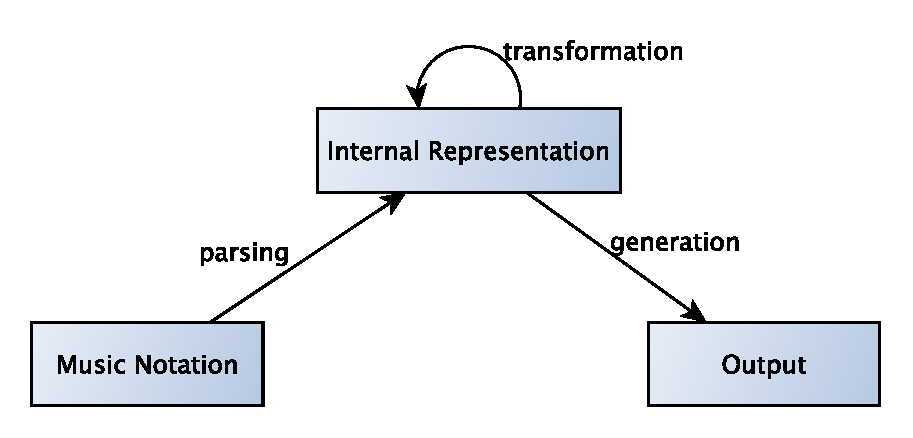
\includegraphics[width=0.8\textwidth]{img/abc_dt.pdf} 
  \caption{\abcpt{} architecture}
  \label{fig:process_stages}
\end{figure}

In order to generate a specific tool, we only need to build the stages - 2) and 3) - that depend on
the rules.

% From figure \ref{fig:process_stages}, we can see that \abcdt{}'s processor behaves like an \abc{}
% compiler generator tool.

\subsection{Parse ABC Input} 

    As previously stated in the introduction, we want to be able to deal with real \abc{} music.
    The \abc{} parser has to be robust, i.e., to be able to expect cases that it doesn't recognize.

    % Also, its implementation must be easy and fast.

    The main options for building the parser were: to build it from scratch; to reuse an existing
    parser from robust programs like \abcmtops{} or \abctomidi{} and adapt it to the requirements;
    or to use directly one of the aforementioned programs' parsers.

    Since building a robust parser is very time consuming, the first solution was discarded. The
    second option would raise problems when adapting our parser to newer versions. So, \abcmtops'
    parser was the natural choice.

\subsubsection{\abcmtops{} parser's features} 

    \abcmtops{} is one of the most widely used programs for working with \abc, not just as a
    standalone software but as part of many applications. This fact implies that it's not a piece of
    software that was casually made. It was designed to process \abc{} in the best way possible,
    therefore its quality is acknowledged.

    It is actively maintained and well documented which facilitates the analysis of the structures
    it generates. Moreover, its author, Jeff Moine, was and still is a preponderant influence for
    the evolution of the \abc{} notation and standard.\\

    The IR generated by its parser follows the sequential structure type, in other words, each
    element captured by the parser is simply appended to an ordered list. An element is any
    component existing in \abc{}, from the header information - like the key or initial meter - to a
    note, bar or a tuplet. The processor that will go through the structure has to keep record of
    the context of each element. The context comprises components like the voice, the meter, the
    length, the key, among others...\\

    % After an initial analysis, the IR's structure revealed itself as being very
    % rich with information from the original \abc source, holding every single piece of information.

    Given that \abcmtops{} was designed to print \abc{}, its IR is not suited for music analysis or
    composition purposes. Therefore, it lacks all the benefits inherent to an hierarchical
    representation, such as, inheriting behavior and characteristics between musical events.

    Still, it can be easily organized as a set of monophonic voices. This set might, for instance,
    be used as a starting point to describe relationships between vertical musical entities on a
    polyphonic score.\\

    As the aim of this work is to build a toolkit based on scripts, the sequential structure reveals
    itself as an appropriate structure that meets our requirements.
    
    The sequence of elements that the structure provides can be easily mapped to an array or a hash.
    These data types are part of the common, yet powerful, data types of a scripting language like
    Perl, which is exactly what we want.

\subsubsection{From \abcmtops{} parser's IR to Perl}

    \abcmtops's parser is implemented in C, so the structure that it generates (a list of C data
    structures) has to be adapted to Perl. This adaptation is done by a Perl
    serialization\footnote{Serialization is the process of translating data structures into a format
    that can be stored and resurrected later in the same or another computer environment.} process
    of the original C structure. Hence, we've created a program - called \emph{C2Perl} - that parses
    an \abc{} file, transforms the generated C structure and prints the serialized Perl output.\\
    
    In short, \emph{Parse \abc{} Input} stage is comprised of a Perl serialization of \abcmtops{}'s
    parser generated structure followed by a Perl evaluation of the serialized structure into a Perl
    \emph{hash}. This way, we obtain a Perl structure that maps the original C structure.\\

    Figure \ref{fig:parse_abc_input_stage} depicts the internal workflow of the \emph{Parse \abc{}
    Input} stage. \emph{C2Perl}'s workflow is represented by the group node '\emph{C2Perl}'.

    \begin{figure}[htb]
      \centering 
      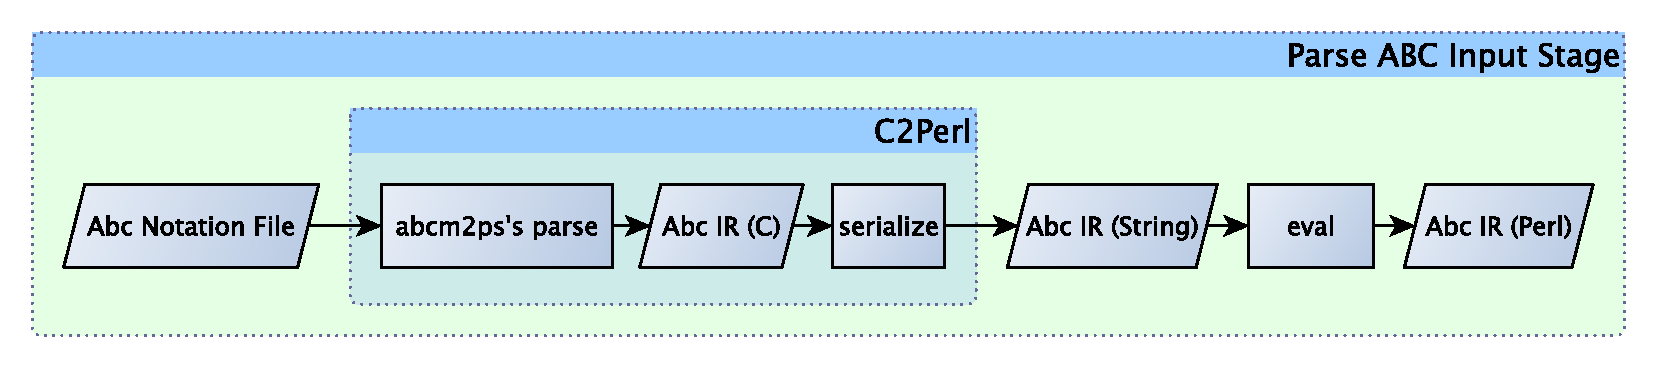
\includegraphics[width=\textwidth]{img/parse_abc_input_stage.pdf} 
      \caption{\emph{Parse \abc{} Input} stage}
      \label{fig:parse_abc_input_stage}
    \end{figure}

    We are merely mapping the original C structure to a Perl one, thus keeping the original order
    and meaning. However, it could be possible to reorganize the structure in order to serve other
    purposes. For example, organize it as being oriented to the part, meaning that we could access
    directly to a specific part. Or organize it by elapsed time, meaning that it would be possible
    to retrieve all events that occurred in a specific moment in time.

\subsection{Transform the generated representation}

    This stage's process - \abcprocessor{} - makes an IR traversal applying the \abcdt{} rules to
    each element.

    The generic processing strategy is to provide a set of transformations for very specific points
    (defined by actuators) and through that obtain the general tools. Any point not covered by the
    rule's actuators is kept unchanged, following the default transformation which is the identity
    function.

    This kind of strategy is effective in building tools that do simple transformations - we only
    need to provide what is to be changed.

\subsubsection{ABC::DT Rules}

    \abcdt{} rules - \texttt{handler} - are defined by a correspondence between an actuator and a
    transformation. An actuator selects a specific element - like a note - or a set of elements -
    like all elements that are defined in a particular context/state. Each actuator is translated
    into an expression that matches different element attributes, in order to accurately select it.

    The actuators enable the existence of different levels of detail that guide the search for the
    required element. Thus, the actuator has a natural notation, in which, more generic elements are
    written before more specific ones. The elements within an actuator are separated by the
    characters '\texttt{::}'.

    For example, '\textit{in\_line::K:}' selects all key elements (K) with state 'in\_line', that
    is, a key which is defined after the header and is surrounded by square brackets -
    \texttt{[K:G]}. Another example, '\textit{note::!f!}' selects all note elements which have the
    decoration \texttt{!f!} associated - \texttt{!f!G}.

    Due to the existence of different levels of detail, when there is more than one actuator that
    matches an element, the most specific is the one applied to the element.

    In \abcdt{} rules, the user can define a special actuator called \emph{-default} to describe how
    to transform each uncovered element. Optionally, a \emph{-end} actuator can be defined, which
    enables a general post processing of the final \abc{}, hence, making possible to attain
    different output formats.

\subsubsection{Processor Algorithm}

    \abcprocessor{} is guided by the IR's structure, meaning that each element is processed
    sequentially. It admits a table of rules, called \texttt{handler} - a dispatch table\footnote{A
    dispatch table is a table of pointers to functions or methods.} - in which an actuator is
    associated with a transformation. During the structure's traversal, when an element matches an
    actuator, the corresponding transformation is applied. An actuator selects a specific element or
    a group of elements. A transformation is specified by the user and it defines how each element
    should be processed according to its internal values.\\

    % Its behavior resembles the one from the utility \awk, in which text files are processed and each
    % file is transformed into a sequence of symbols. The processing is based on a sequence of
    % pattern-action statements. Each symbol is processed one at a time and matched against each
    % pattern, and for each pattern that matches, the associated action is executed.\\

    This implementation's main features are:
    \begin{description}
      \item[Dispatch Table] \hfill \\
        \abcdt{} rules are defined by a correspondence between the actuators and transformations,
        called \texttt{handler}.
      \item[Higher-Order Processing] \hfill \\
        The transformations are user specified functions.
      \item[Systematic] \hfill \\
        In order to build a tool, a user must define what and how is to be transformed.
      \item[Specify only the necessary] \hfill \\
        If no actuator applies, the identity function is used.
      \item[Rich Actuators] \hfill \\
        The set of actuators is comprised of well structured elements in order to provide a precise
        processing.
      \item[Processing strategies] \hfill \\
        There is a table of strategies. Each strategy defines how a transformation's output is to be
        merged with others. 
    \end{description}

    During the traversal, \abcprocessor{} calculates the current element's state, including the
    voice id, the time elapsed per voice. That state grants a more complete control of what can be
    processed and provides a richer semantic processing.

    % In order to define how the outcome of processing a symbol should be merged with others, the
    % processor must know which processing strategy it must use. Thus, a table of strategies is needed
    % and by default the processor uses the \texttt{STR} strategy which makes the string concatenation
    % of the outcome of each symbol.\\
    %TODO nao sei se consegui fazer sentido. consultar tese jj
    % Other strategies might be added to the table. For instance, a strategy that maps a set of
    % symbols to a Perl structure so that it can be processed as a whole. Such a set might be
    % difficult to process with the default strategy.

    The processor's algorithm was inspired in the one used in XML::DT~\cite{tesejj}, a processing
    module of XML documents.

\subsection{Generate the output}

    In this stage, the transformed representation is outputted and it may be of the same type as the
    input, which enables the composition of other tools.

    The identity function, which is called \toabc, prints the contents of an element just as they
    were in the \abc{} source tune. This function's implementation was based on the one used by
    \texttt{tclabc}~\cite{tclabc:Online} which also uses \abcmtops' parser.

\section{ABC::DT by example}
\label{sec:abc_dt_by_example}

In this section we will present examples of tools created using \abcdt{},
thus demonstrating how easily a (simple) tool or some occasional processing can be made. 

\subsection{All But One}

    When there is a multi-voice score, like a four part choir, it is important to, for instance, the
    Soprano to hear all the other parts except hers.  That way, she can study her part knowing what
    the rest is going to sound.

    The \emph{All-but-one} tool generates an \abc{} score whose goal is to help musicians in
    individual rehearsal of multi-voice music for studying purposes. 

    In \abc{}, it is possible to add commands to control audio properties. \abctomidi{} recognizes
    \midi directives -- \emph{\%\%MIDI}, followed by different parameters. For \emph{All-but-one},
    we need to add a \midi directive to reduce the volume of the voice. To be more precise, it has
    to generate a change-volume \midi directive -- \emph{\%\%MIDI control 7 NewVolume}, where
    NewVolume is a number between (0-127) -- after the voice definition for it to be silenced.\\

    % This tool generates an \abc{} score whose goal is to help musicians in music learning and
    % studying. That is, when there's a score with more than one voice, like a four part choir score,
    % it is important to, for instance, the Soprano to hear all the other parts except hers. That way,
    % she can study her part knowing what the rest is going to sound.

    % In \abc, this is possible by adding to the tune a command that controls audio effects.
    % \abctomidi{} provides such commands by means of the meta-comment \emph{\%\%MIDI},
    % followed by different parameters. In this tool's case, the only \abctomidi{} command
    % needed is \emph{\%\%MIDI control}, which generates a \midi control event. To be more precise, it
    % has to generate the \midi command that controls the main volume, that is, \emph{\%\%MIDI control
    % 7}, followed by the volume's value itself, which is a number between (0-127).\\
    % Therefore, it's only required that the \midi command be appended after the voice statement.

    This command line program, may receive command line options:
    \begin{description}
      \item[-v, --voice] \hfill \\
        A string is expected identifying either the voice's id - a number generated by the parser -
        or name that will be attenuated.
      \item[-m, --min-volume] \hfill \\
        A number is expected defining the volume's value for the voice to be attenuated.
    \end{description}

    The \abcdt{} specification is quite simple. There is only one rule: selecting the
    voice to be attenuated, and add a change-volume command, as illustrated in listing \ref{lst:handler}.\\

    \lstinputlisting[caption={Handler},label={lst:handler},captionpos=t,abovecaptionskip=-\medskipamount]{misc/handler.tex}

    The variable \texttt{\$requested\_voice} is defined by the command line option. So, if
    \texttt{\$requested\_voice} is "Tenor", the actuator is \texttt{V:Tenor}, and it will search for
    the element \emph{voice} whose name is "Tenor".

    The output of \emph{All-but-one} is an \abc{} tune so it can be chained with other \abc{} tools.

    Listing \ref{lst:abc_all_but_one} shows how this tool could be used. It reads the tune 100.abc
    (listing \ref{lst:verbum_s1}) and the output is
    shown in listing \ref{lst:100_all_but_tenor}.\\

    \lstinputlisting[caption={\abc{} All But One},label={lst:abc_all_but_one},captionpos=t,abovecaptionskip=-\medskipamount]{misc/abc_all_but_one.tex}

    \begin{center}
      \begin{minipage}{.49\textwidth}
        \lstinputlisting[caption={100.abc},label={lst:verbum_s1},captionpos=t,abovecaptionskip=-\medskipamount]{misc/verbum_s1.tex}
      \end{minipage}
      \hfill
      \begin{minipage}{.49\textwidth}
        \lstinputlisting[caption={100\_all\_but\_tenor.abc},label={lst:100_all_but_tenor},captionpos=t,abovecaptionskip=-\medskipamount]{misc/100_all_but_tenor.tex}
      \end{minipage}
    \end{center}

    Note the \midi command \texttt{\%\%MIDI control 7 25} after the voice definition \texttt{V:3
    name="Tenor" sname="T." clef=treble-8}. This way, the voice "Tenor" is going to be attenuated
    when \abctomidi{} reproduces the score.

\subsection{ABC Paste}

This tool, as the Unix Paste, merges the voices of tunes parallel to each other in the time
perspective. In other words, each voice starts at the beginning of the resulting tune.

Some decisions were made regarding what should be done with some information present in a tune. This
ensured that the resulting tune was consistent with each individual tune:

\begin{enumerate}
  \item The context at each point in the tune is recorded. The context comprises the current voice,
    the key, the meter, the length, the tempo and the number of measures for each voice.
  \item Any context change like the key or the meter is written only if it differs from the current.
  \item The resulting tune's header is the one present in the first tune which has an actual tune
    written, in other words, at least one note.
  \item In the resulting tune, any voice that has fewer measures than the longest one is appended
    with measure rests.
\end{enumerate}

The tool's algorithm is divided in three stages: 1) retrieving the header for the resulting tune, 2)
pasting the tunes and 3) appending any necessary rests.\\

\textbf{1)} As mentioned before, the resulting tune's header is the one from the first tune with at
least on note written. This follows a simple algorithm where each tune is searched in the order they
are passed in. As soon as it finds a tune with a note written it stops, following to the next step.
The \texttt{handler} to be passed to the processor needs only three entries, each corresponding to a
tune's state that the \abcmtops' parser generates.

\textbf{2)} Pasting is the most complicated part, yet in the end it was not that difficult to
implement. The algorithm consists on running the processor for each tune and concatenating each
result.\\
The handler has some entries like the one in listing \ref{lst:counting_measures}, where everytime
the element corresponding to the measure bar is visited, a counter for the current voice's written
measures is incremented. The identity function \toabc{} is called so that the actual bar
can be outputted.
\lstinputlisting[caption={Counting measure bars},label={lst:counting_measures},captionpos=t,abovecaptionskip=-\medskipamount]{misc/counting_measures.tex}
Other entries update the current voice variable when a \textit{voice} is found or the current key
when a \textit{key} is found. Through the context variables, which are constantly updated, it is
possible to compare the current context and the new. This enables the possibility of not printing the
context declaration if it is the same as the current, thus making the resulting tune cleaner without
useless duplications.

\textbf{3)} The final step happens after step 2) and it consists on verifying if there is any voice
with fewer measures than the voice with the biggest number of measures. If there is such a voice
then a multiple measure rest with the difference is appended to that voice. This is possible
because, in step 2), the number of measures for each voice was being recorded.

In the end the output generated is printed to the output. Since it is still an \abc{} tune it can
be the input of other tools like this one or \abc{} Cat that will be described next.\\

Listing \ref{lst:abc_paste_by_example} shows how this tool could be used. It reads tunes 101.abc
(listing \ref{lst:verbum_s1_p1}) and 103.abc (listing \ref{lst:verbum_s1_p3}) and the output is
shown in listing \ref{lst:verbum_s1_p1_p3_pasted} with its respective score (figure
\ref{fig:verbum}, area A).

\lstinputlisting[caption={\abc{} Paste by example},label={lst:abc_paste_by_example},captionpos=t,abovecaptionskip=-\medskipamount]{misc/abc_paste_by_example.tex}

\lstinputlisting[caption={Verbum caro factum est: Section 1; Part 3 - Tenor},label={lst:verbum_s1_p3},captionpos=t,abovecaptionskip=-\medskipamount]{misc/verbum_s1_p3.tex}

\vspace{-1.30cm}
\begin{center}
  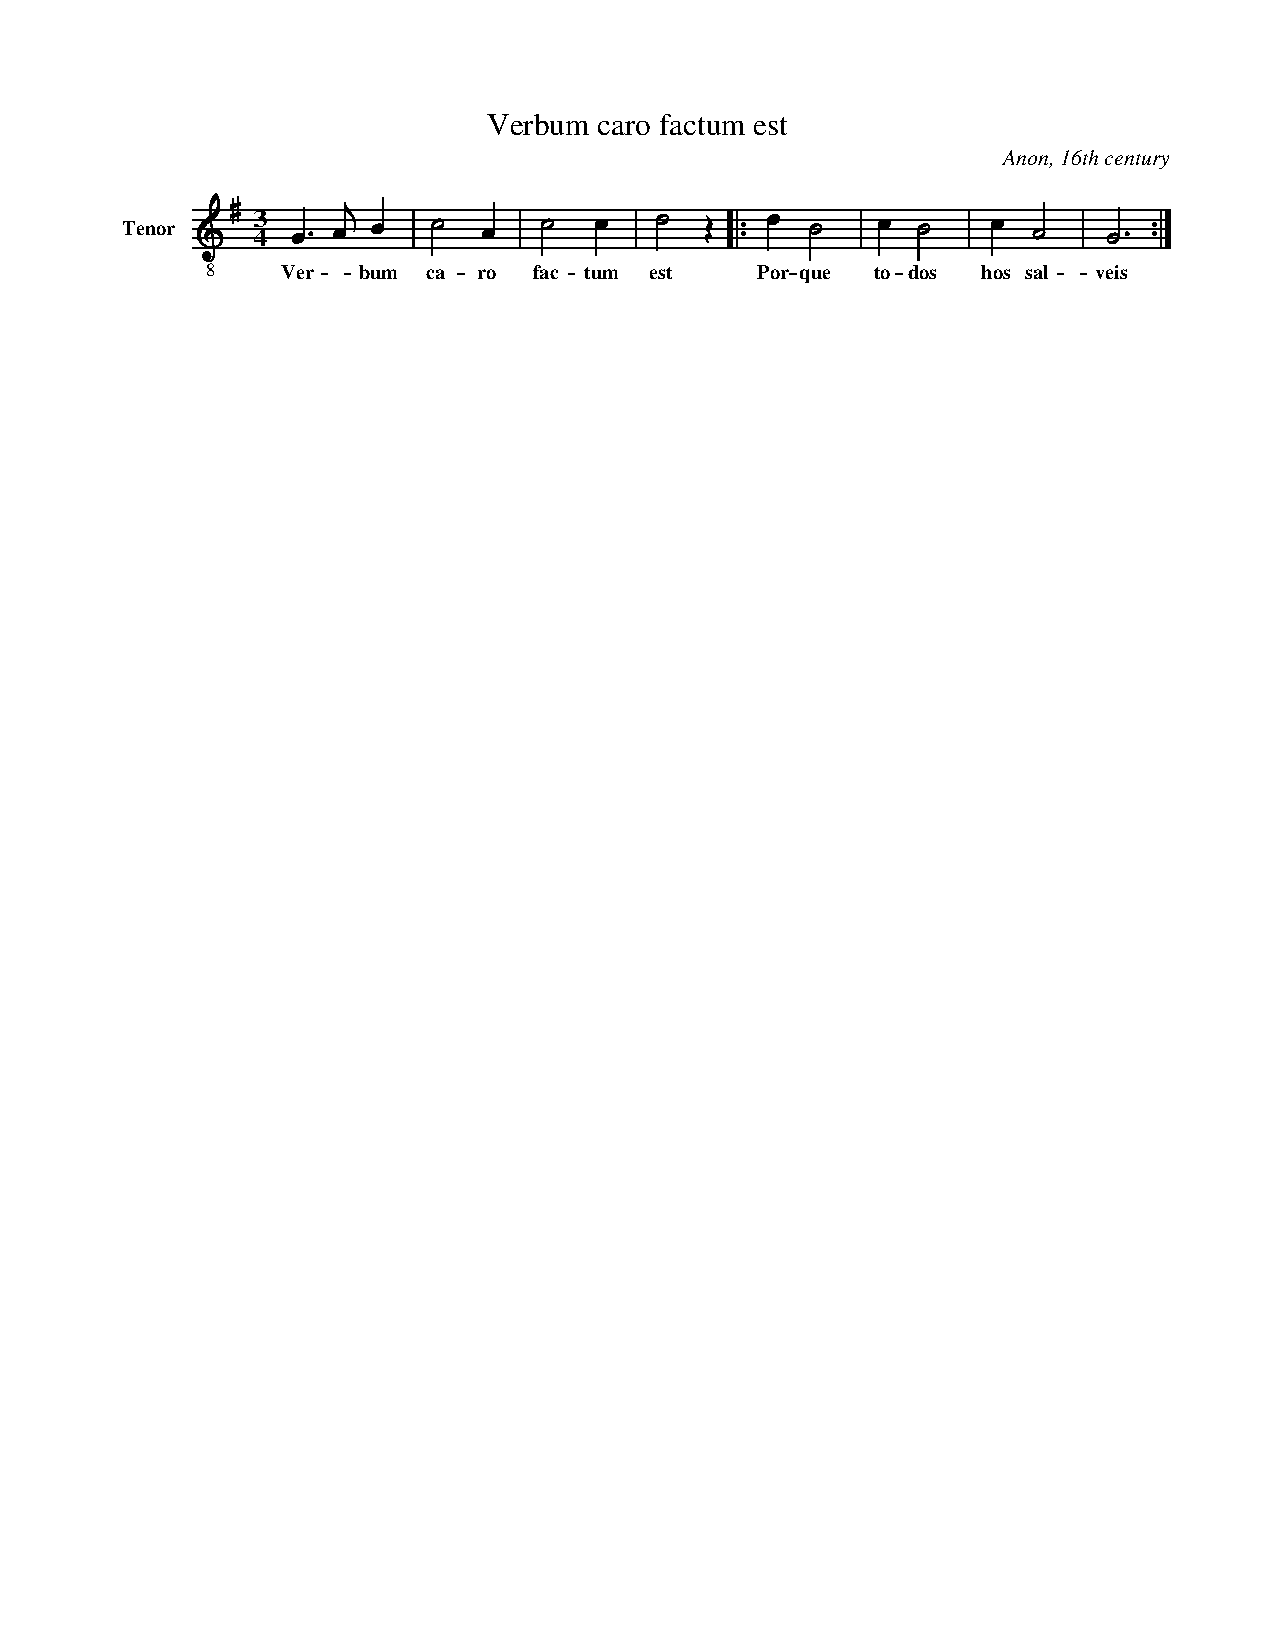
\includegraphics[width=0.8\textwidth, clip=true, trim = 15mm 231mm 0mm 0mm]{img/103.pdf} 
\end{center}

\lstinputlisting[caption={Verbum caro factum est: Section 1; Part 1 \& 3},label={lst:verbum_s1_p1_p3_pasted},captionpos=t,abovecaptionskip=-\medskipamount]{misc/verbum_s1_p1_p3_pasted.tex}

\subsection{ABC Cat}

This tool is based on Unix's cat, as it consists on the concatenation of each tune one after the
other in the time perspective. In other words, any voice present in the second tune is always
printed after any voice present or not in the first, and so on.

Some design goals were established:

\begin{enumerate}
  \item The context at each point in the tune is recorded. The context comprises the current voice,
    the key, the meter, the length, the tempo. The number of measures for each voice is recorded
    separately for each tune.
  \item Any context change like the key or the meter is written only if it differs from the current.
  \item Each tune's header information regarding the tune's context is always written except if it
    is the same as the current one.
  \item For each tune, before printing it, a verification for missing voices is made in the current
    tune and all prior to that. This way, measure rests can be appended in order to have a
    consistent resulting tune.
  \item Any voice that has fewer measures than the longest one will be appended with measure rests.
\end{enumerate}

The tool comprises only one step. Yet it is more complex than \abc{} Paste's.\\
Its algorithm consists in traversing all tunes, running the processor for each tune and verifying if
there are any measure rests to append to a voice. This is done by comparing voice's measures within
the current tune and previous ones.\\
The \texttt{handler} is very similar to the one used in \abc{} Paste.

In the end the output generated is printed to the output. Since it is still an \abc{} tune it can be
the input of other tools.\\

Listing \ref{lst:abc_cat_by_example} shows how this tool could be used. It reads tunes 201.abc
(listing \ref{lst:verbum_s2_p1}) and 303.abc (listing \ref{lst:verbum_s3_p3}) and the output is
shown in listing \ref{lst:verbum_s2_p1_s3_p3_cated} with its respective score (figure
\ref{fig:verbum}, area B).

\lstinputlisting[caption={\abc{} Cat by example},label={lst:abc_cat_by_example},captionpos=t,abovecaptionskip=-\medskipamount]{misc/abc_cat_by_example.tex}

\lstinputlisting[caption={Verbum caro factum est: Section 2; Part 1 - Soprano},label={lst:verbum_s2_p1},captionpos=t,abovecaptionskip=-\medskipamount]{misc/verbum_s2_p1.tex}

\vspace{-1.30cm}
\begin{center}
  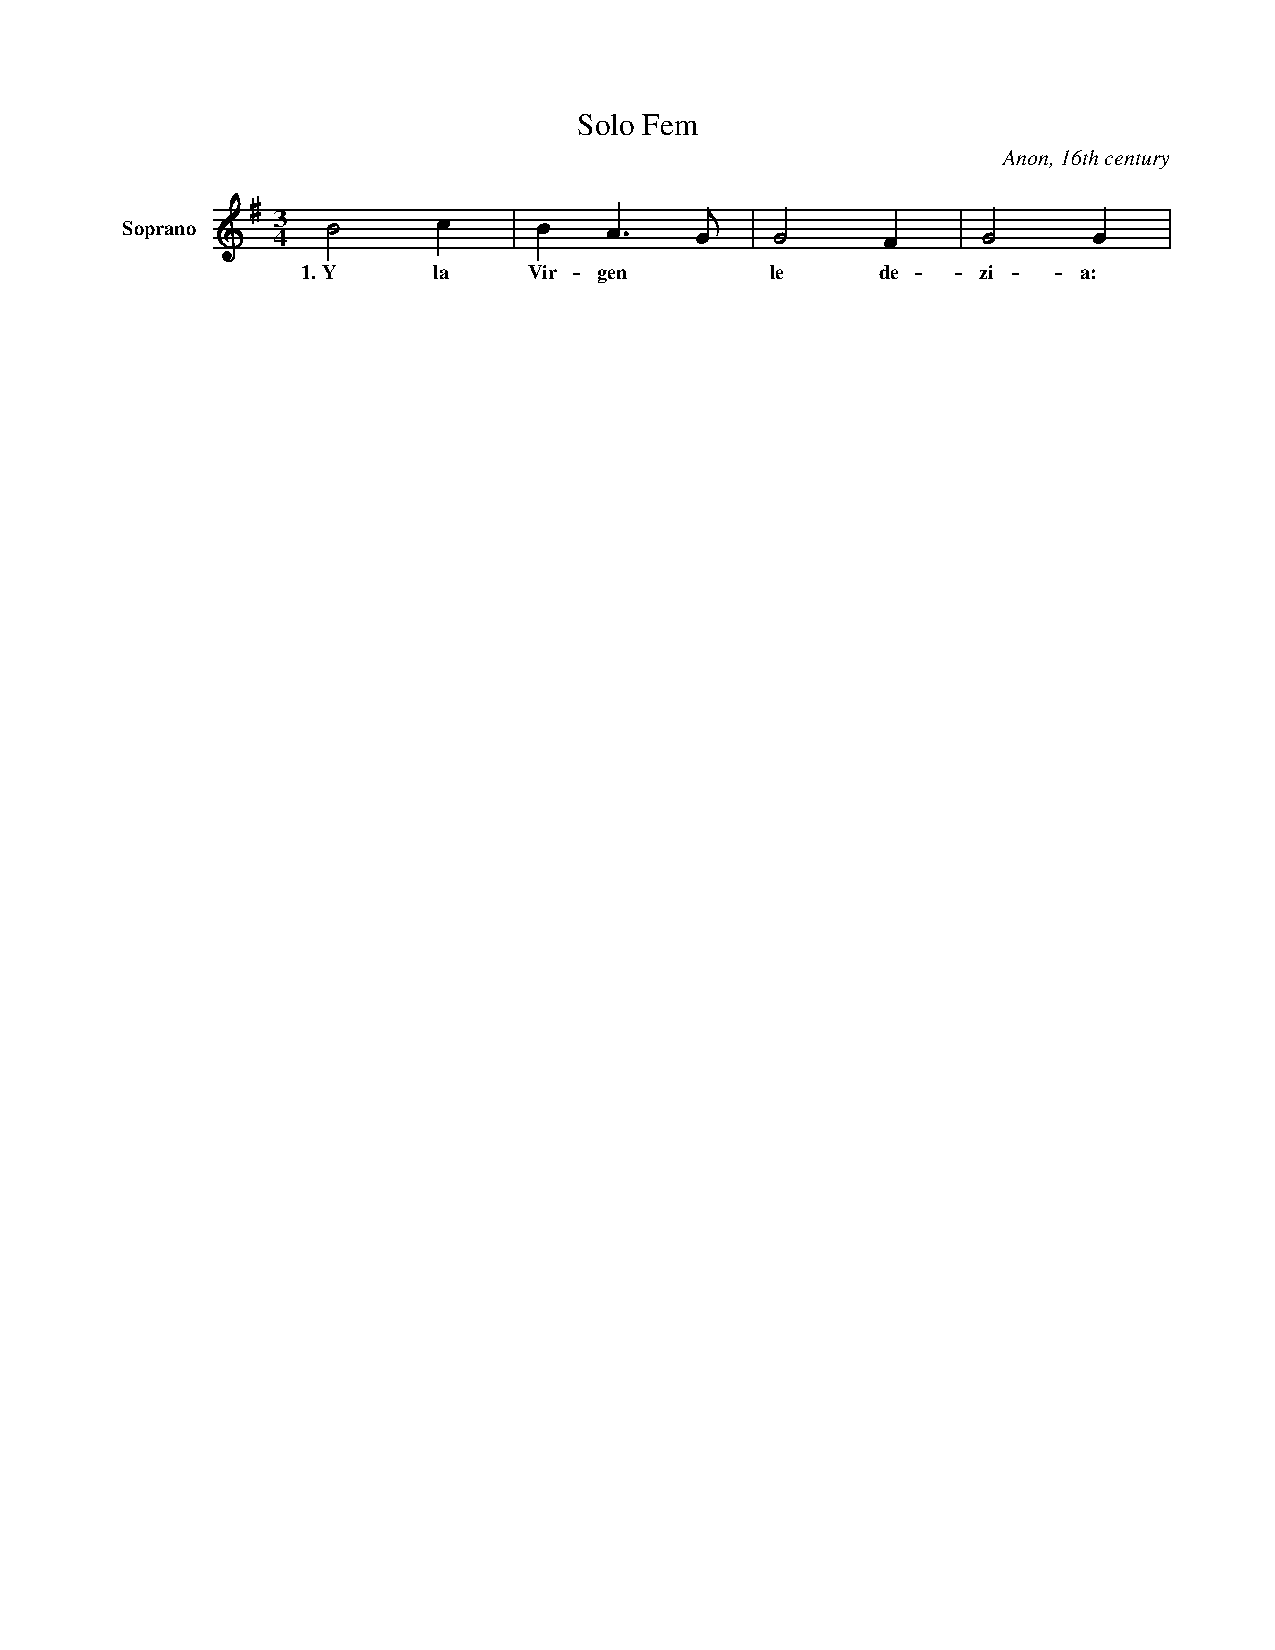
\includegraphics[width=0.8\textwidth, clip=true, trim = 15mm 231mm 0mm 0mm]{img/201.pdf} 
\end{center}

\lstinputlisting[caption={Verbum caro factum est: Section 3; Part 3 - Tenor},label={lst:verbum_s3_p3},captionpos=t,abovecaptionskip=-\medskipamount]{misc/verbum_s3_p3.tex}

\vspace{-1.30cm}
\begin{center}
  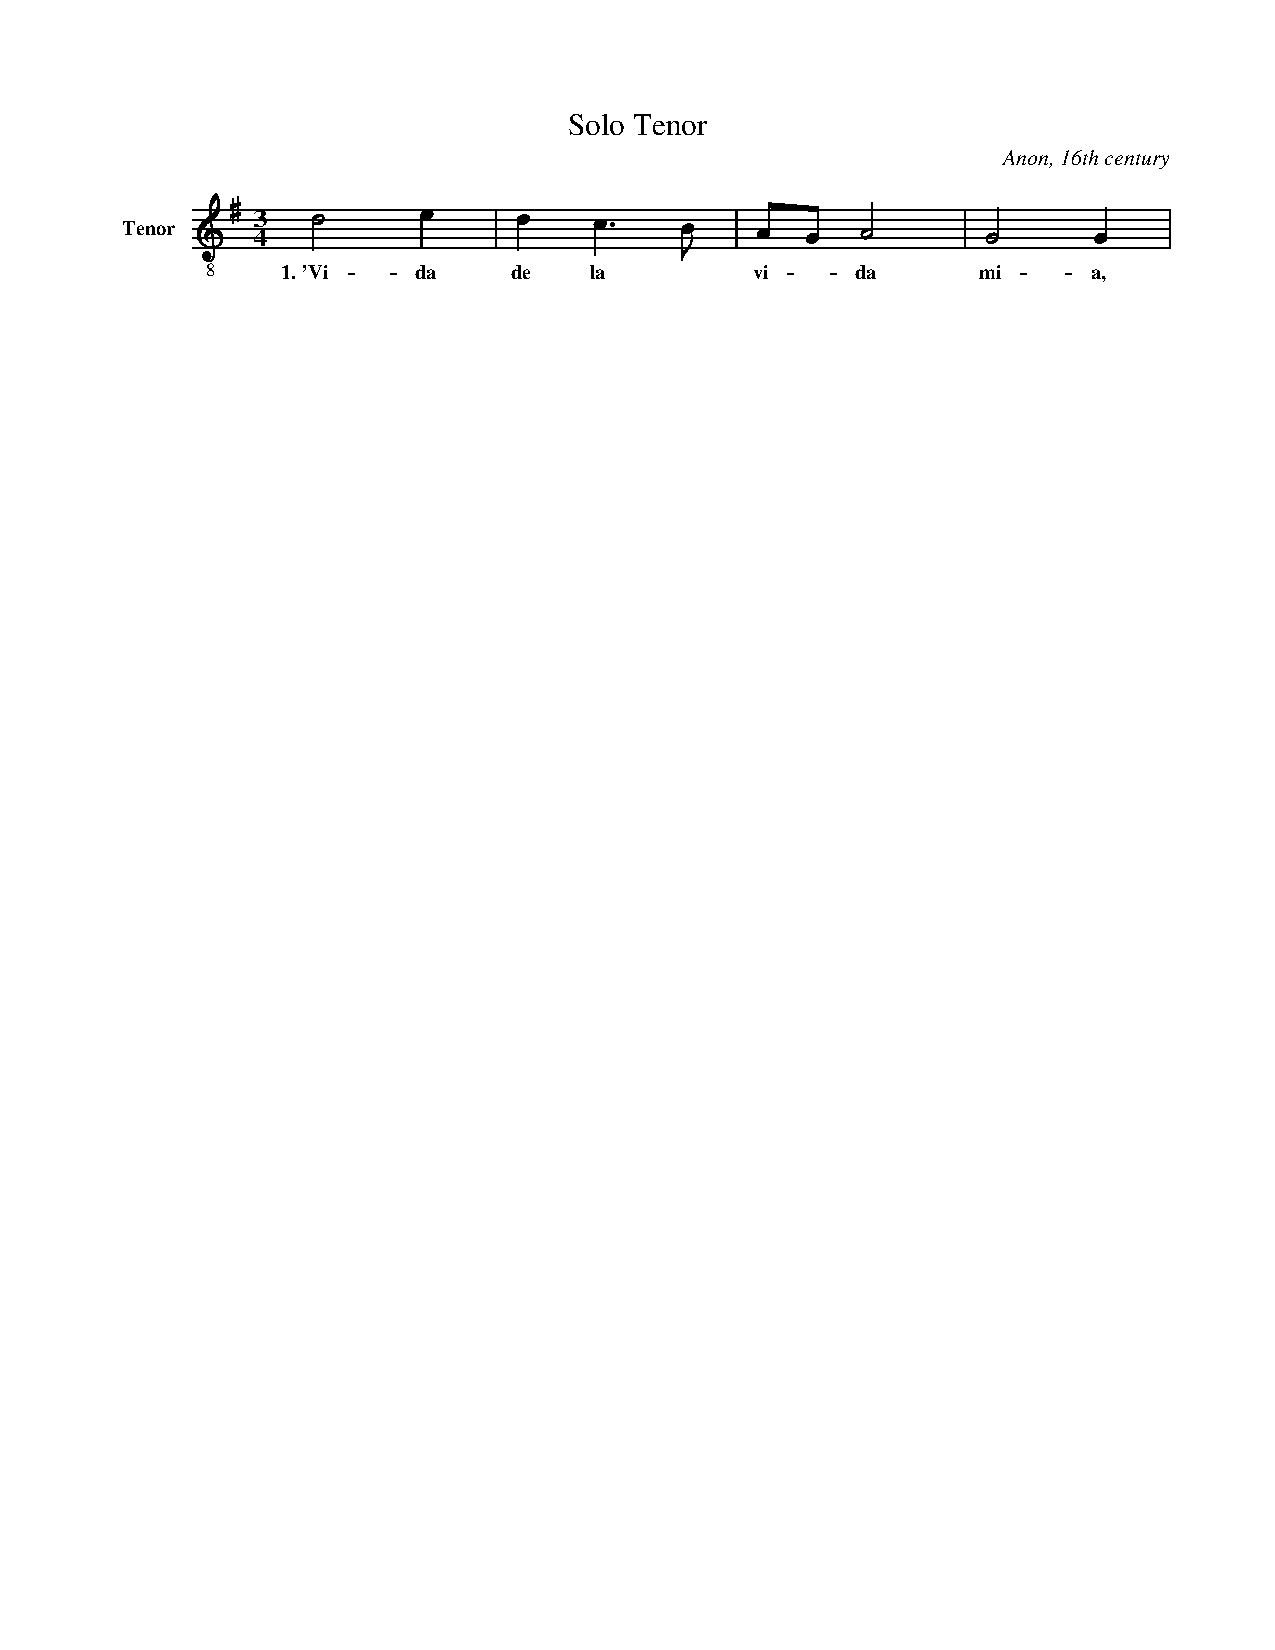
\includegraphics[width=0.8\textwidth, clip=true, trim = 15mm 231mm 0mm 0mm]{img/303.pdf} 
\end{center}

\lstinputlisting[caption={Verbum caro factum est: Section 2: Part 1 \& Section 3: Part 3},label={lst:verbum_s2_p1_s3_p3_cated},captionpos=t,abovecaptionskip=-\medskipamount]{misc/verbum_s2_p1_s3_p3_cated.tex}

\subsection{Real Example}
A real application for these tools could be their composition. Using the score \textit{Verbum caro
factum est} whose sections and parts are divided in separate files, it is possible to assemble the
whole score by composing \abc{} Paste with \abc{} Cat. The score will be composed by the examples
shown previously, so it will be comprised of three sections and only two parts (Soprano and Tenor).
Listing \ref{lst:cat_paste_by_example} shows how the tools are composed and listing \ref{lst:verbum}
shows the \abc{} for the composed score.

\lstinputlisting[caption={\abc{} Cat and Paste by example},label={lst:cat_paste_by_example},captionpos=t,abovecaptionskip=-\medskipamount]{misc/cat_paste_by_example.tex}

\lstinputlisting[caption={Verbum caro factum est: Sections 1, 2 \& 3; Parts 1 \& 3},label={lst:verbum},captionpos=t,abovecaptionskip=-\medskipamount]{misc/verbum.tex}

\vspace{-1.30cm}
\begin{figure}[htb]
  \centering 
  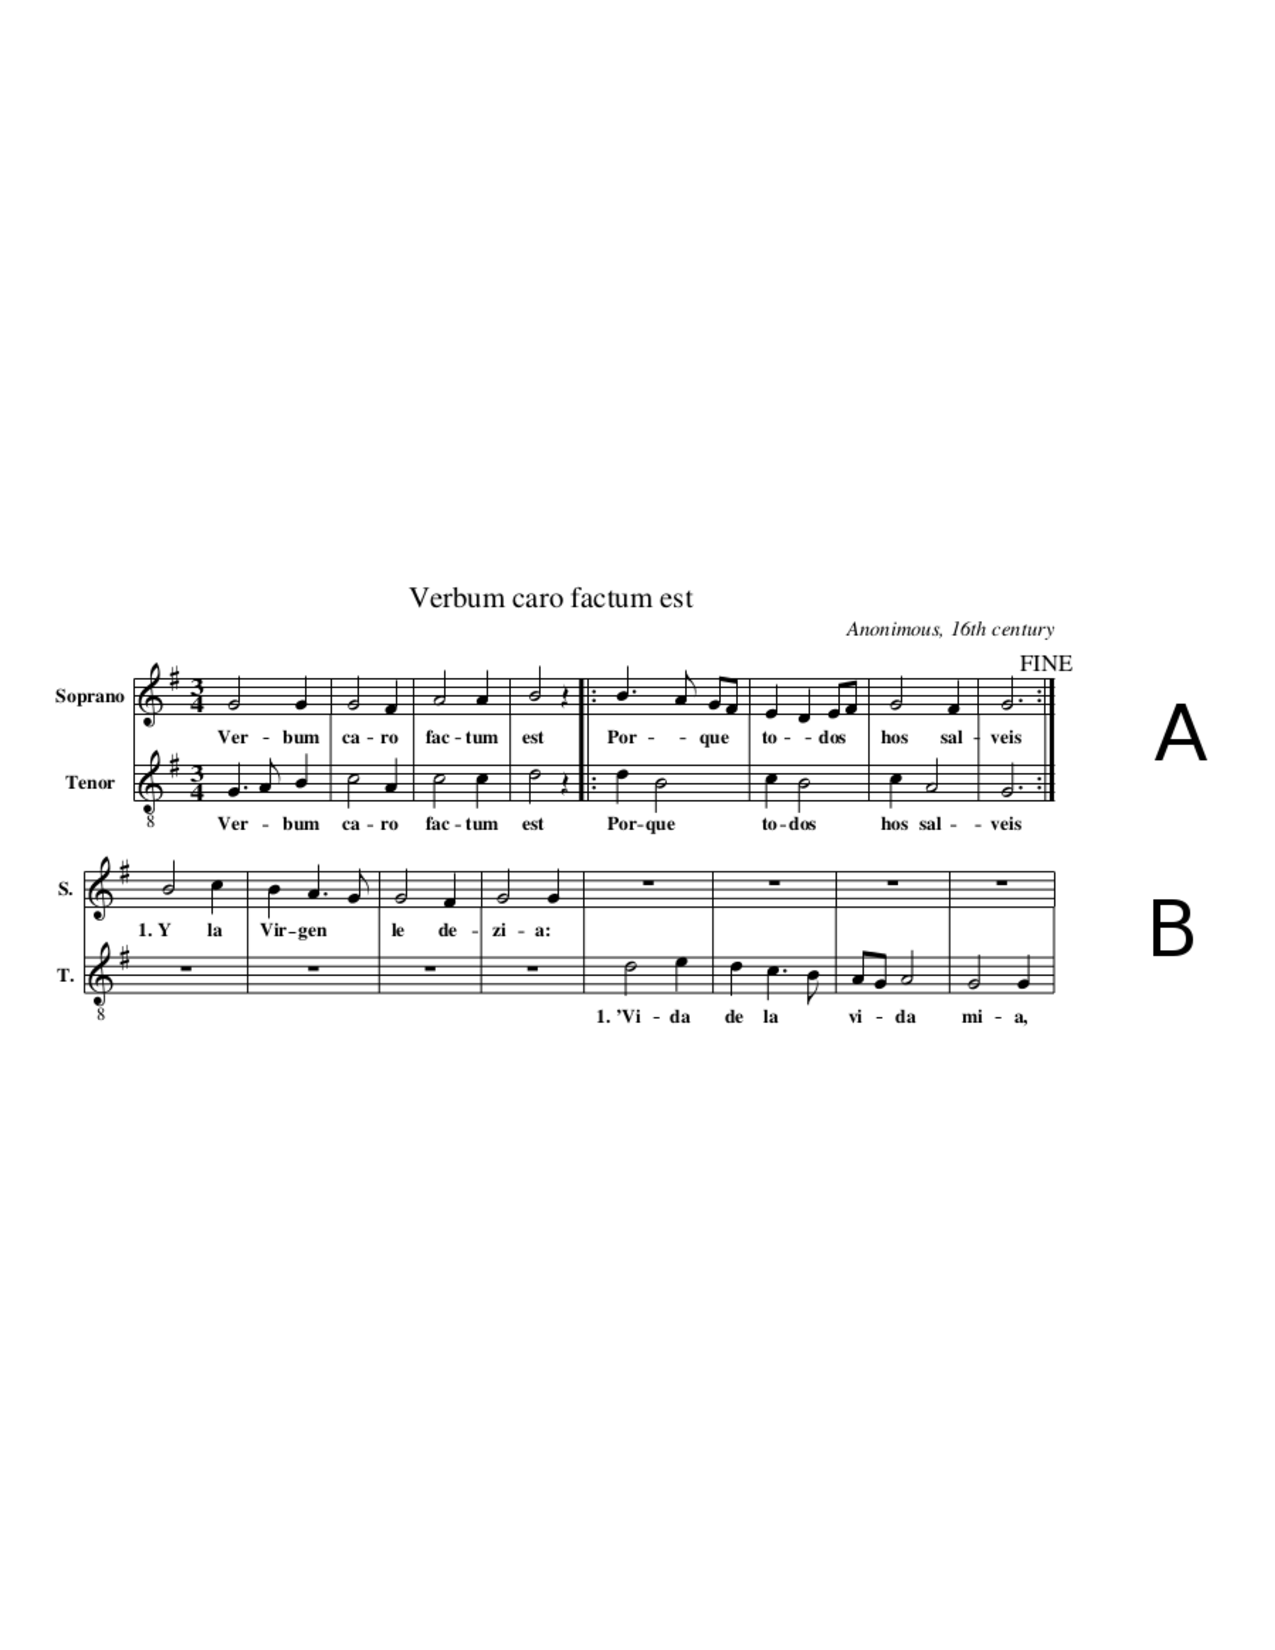
\includegraphics[width=0.8\textwidth, clip=true, trim = 0mm 105mm 0mm 76mm]{img/c_letters.pdf} 
  \caption{Verbum caro factum est Score: Sections 1, 2 \& 3; Parts 1 \& 3}
  \label{fig:verbum}
\end{figure}

\section{Conclusions}

Inspired in a solution that revealed successful - the creation of the language C to help developing
Unix - a DSL, called \abcdt{}, was created in this work as well.

Reusing \abcmtops{}'s parser was very important to help guarantee this work's quality, coverage and
developing time. The generated IR is source oriented which allows obtaining valid \abc{} and robust
tools - it knows how to deal with unknown elements.

The representation used must be complete enough to enable the application of many different analytic
tasks. However, that fact doesn't invalidate an approach that starts by generating a sequential
structure and from it generating something more suited to more complex uses.

Using Perl as the language embedded into \abcdt{} provides a rich environment to allow easy
processing of text. Furthermore, through the use of data structures, like hashes, the user has
bigger expressive power to specify transformations.

We believe that the rule based processor makes it possible to write very compact tools.

One of our main goals is to build an \abc{} operating system. Moreover, presently, there is a lack
of music notation general processing tools, particularly for \abc{}. Thus, the existence of DSL's
like \abcdt{} helps to the simplification of crafting new \abc{} processing tools.

%%
%% Bibliography
%%
% \nocite{*}
%TODO JJ validar refs uma a uma
\bibliography{bib/article}

\end{document}
